%%
%% Capítulo 2: Desenvolvimento do trabalho
%%

\mychapter{Desenvolvimento}
\label{Cap:desenvolvimento}

Este capítulo apresenta considerações de ordem geral sobre a
organização e desenvolvimento do texto.

\section{O que escrever}
\label{Sec:oque}

É possível iniciar o capítulo de desenvolvimento informando como será desenvolvido o trabalho e o detalhe das ferramentas ou o conteúdo que será abordado e utilizado. Em seguida comente o conteúdo em conjunto com o conhecimento adquirido junto as consultas e referências bibliográficas. 
Isso demonstra que foi feito uma pesquisa anterior e mostra que o trabalho tem relevância científica, ou seja, não está sendo "inventada a roda". 

\section{Divisões do documento e referências cruzadas}
\label{Sec:divisoes}

Sempre que for modificar/aprofundar partes de um tema, é interessante criar uma seção de maneira a tornar o assunto mais focado e facilitar a leitura. 
Não crie seções sem que estas tenham nenhum texto ou sigam direto para outra seção. Se isso acontecer é melhor rever como está organizado o texto pois pode se tornar necessário remover capítulos ou seções. 

No final de cada capítulo é importante apresentar comentário do que foi desenvolvido no texto permitindo ao leitor compreender a visão geral do conteúdo e pode-se inclusive contextualizar o capítulo seguinte.



\mychapter{Figuras, tabelas e gráficos}
\label{Cap:figuras}

Uma das maiores dificuldades na edição de textos de qualidade é o
posicionamento dos elementos gráficos: figuras, gráficos e
tabelas. Como estes elementos muitas vezes são grandes, aparece o
dilema sobre o que fazer quando uma quebra de página deveria acontecer
no meio do elemento. Há duas possibilidades:
\begin{enumerate}
\item O autor informa exatamente onde o elemento gr‡fico deve ficar no
texto, evitando que quebras de páginas aconteçam no meio de um
elemento. O problema com esta abordagem é que todo o trabalho de
posicionamento pode ser perdido caso se inclua ou se exclua algum
texto ou elemento.
\item O editor de texto posiciona os elementos gráficos de forma a não
deixar espaços em branco nas páginas. Estes elementos que podem ser
posicionados pelo editor são conhecidos como \emph{elementos
flutuantes}. O problema com esta abordagem é que o posicionamento
adotado pode não corresponder às expectativas do autor.
\end{enumerate}



\section{Tabelas em \LaTeX}
\label{Sec:tabelas}

Tabelas são construpídas com comandos próprios do \LaTeX, notadamente o
ambiente \texttt{tabular}. Nada obriga a que o ambiente
\texttt{tabular} esteja sempre posicionado em um elemento
flutuante. Se você quiser impor que uma tabela fique obrigatoriamente
em uma determinada posição do texto, basta não colocar o
\texttt{tabular} dentro de um \texttt{table}. Tabelas podem até ser
incluídas no meio de uma frase.  Por exemplo, eu posso dizer que se um
jogo da velha está na configuração \textsf{\tiny\begin{tabular}{c|c|c}
x & & x \\ \hline & & o \\ \hline x & o & \end{tabular}} e se o
jogador ``\textsf{x}'' sabe jogar, ent‹o o jogador ``\textsf{o}'' irá
perder, independentemente da jogada que faça.

 Exemplos de
colunas com diferentes larguras e alinhamentos podem ser vistos na
tabela \ref{Tab:larguracolunas}.

\begin{table}[htbp]
\begin{tabularx}{\linewidth}{|p{3cm}|X|l|} \hline
COLUNA p & COLUNA X & COLUNA l \\ \hline
Largura fixa (não depende do conteúdo) &
Expandível &
Ajustável \\ \hline
Alinhada no topo &
Alinhada à esquerda &
Alinhada à esquerda \\ \hline
\end{tabularx}
\\[0.5cm]
\begin{tabularx}{\linewidth}{|b{3cm}|C|r|} \hline
COLUNA b & COLUNA C (ver \texttt{comandos.tex}) & COLUNA r \\ \hline
Largura fixa (não depende do conteúdo) &
Expandível &
Ajustável \\ \hline
Alinhada na base &
Centralizada &
Alinhada à direita \\ \hline
\end{tabularx} 
\caption{Tabelas com colunas de diferentes larguras e alinhamentos}
\label{Tab:larguracolunas}
\end{table}

\section{Figuras em \LaTeX}
\label{Sec:figuras}

As figuras (imagens, desenhos, gr‡ficos, etc.) devem ser produzidas
por ferramentas externas ao \LaTeX, salvas em um arquivo e inseridas
no texto usando o comando \texttt{includegraphics}. Da mesma forma
que as tabelas, as figuras podem ser flutuantes, caso sejam
inseridas dentro de um ambiente \texttt{figure}, ou ter uma posição
fixa no texto (como aqui: 
\includegraphics{figuras/eu}).

O formato em que você deve salvar os arquivos das figuras para que
possa incluí-las no texto depende de como você pretende compilar
o código fonte:
\begin{itemize}
\item se o texto vai ser compilado com \texttt{latex}, todos os
arquivos devem estar no formato EPS (\emph{Encapsulated PostScipt});
\item se o texto vai ser compilado com \texttt{pdflatex}, os
arquivos devem estar nos formatos PDF ou JPEG (outros formatos são
aceitos, mas estes são os recomendáveis).
\end{itemize}

A figura \ref{Fig:belmonte} mostra um exemplo de inclusão de uma
imagem EPS no texto \LaTeX.

\begin{figure}[htbp!]
\begin{center}
% fbox faz uma borda ao redor do seu argumento
\fbox{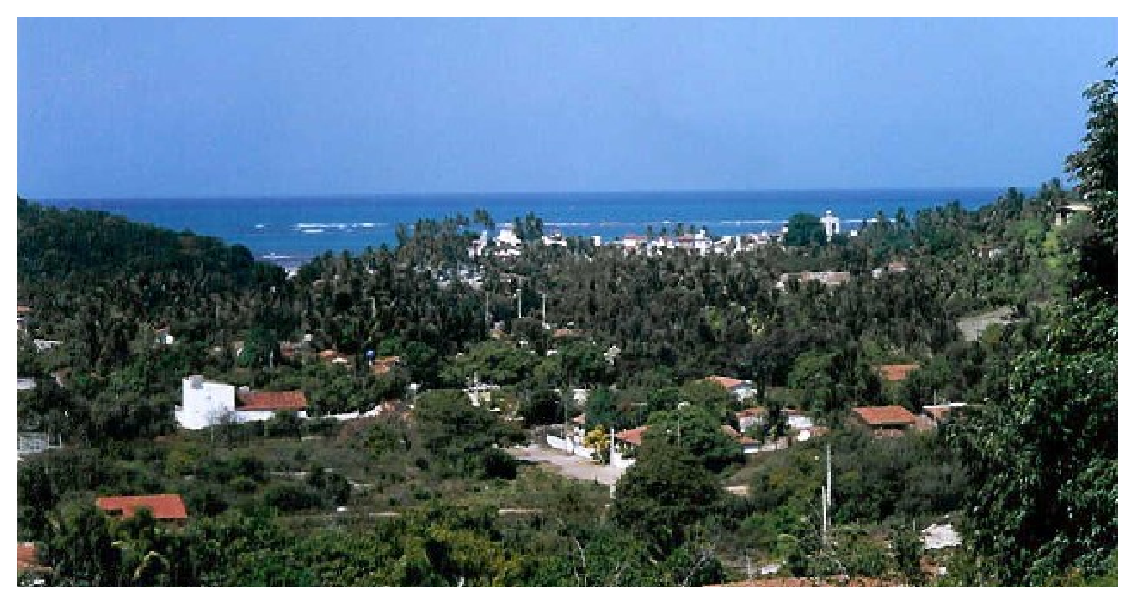
\includegraphics[width=0.75\linewidth]{figuras/belmonte}}
\caption{Exemplo de imagem real}
\label{Fig:belmonte}
\end{center} 
\end{figure}



